\section{Strutture dati per la RLPBWT}
Assemblando le componenti descritte nella sezione precedente, si ottengono otto
varianti della $\RLPBWT$:
\begin{itemize}
  \item due strutture dati composte unicamente dalle componenti dedicate al
  mapping e dall'intero $\RLCP$. Tali strutture sono nominate:
  \begin{enumerate}
    \item[1] \texttt{MAP-INT + RLCP}
    \item[2] \texttt{MAP-BV + RLCP}
  \end{enumerate}
  Queste soluzioni non permettono di sapere quali righe del pannello
  presentino uno $\SMEM$, terminante in una certa colonna, ma solo quante
  esse siano. Non avendo traccia dei valori del prefix array, non si ha modo di
  usare la componente \texttt{PHI}. Il funzionamento dell'algoritmo è basato su
  una re-implementazione 
  dell'algoritmo 5 di Durbin
  \item quattro strutture composte per il calcolo degli $\SMEM$ tramite la
  computazione, 
  in due passaggi, dell'array delle matching statistics, in modo analogo
  a quanto introdotto in MONI \cite{moni} per la $\RLBWT$, tramite
  threshold e random access al pannello. In merito a quest'ultimo, come
  anticipato, si ha che può essere memorizzato come vettore di
  bitvector o come 
  $\SLP$. L'algoritmo  
  necessita, inoltre, sia della componente atta al mapping che di quella
  relativa ai prefix array sample. Infine, per estendere il
  riconoscimento a tutte le righe che presentano un medesimo $\SMEM$ fino ad una
  certa colonna, si necessita della struttura che permette di calcolare le
  funzioni $\varphi$ e $\varphi^{-1}$. Tali strutture sono nominate:
  \begin{enumerate}
    \item[3] \texttt{MAP-INT + THR-INT + RA-BV + PERM + PHI}
    \item[4] \texttt{MAP-INT + THR-INT + RA-SLP + PERM + PHI}
    \item[5] \texttt{MAP-BV + THR-BV + RA-BV + PERM + PHI}
    \item[6] \texttt{MAP-BV + THR-BV + RA-SLP + PERM + PHI}
  \end{enumerate}
  \item due strutture composte per il calcolo degli $\SMEM$ tramite la
  computazione, 
  in un singolo passaggio, dell'array delle matching statistics, in modo
  analogo a quanto introdotto in PHONI \cite{phoni} per la $\RLBWT$, tramite
  l'uso delle $\LCE$ query. Queste ultime sostituiscono l'uso delle
  threshold e del random access al pannello. Tali strutture
  sono nominate: 
  \begin{enumerate}
    \item[7] \texttt{MAP-INT + LCE + PERM + PHI}
    \item[8] \texttt{MAP-BV + LCE + PERM + PHI}
  \end{enumerate}
\end{itemize}
Una visualizzazione grafica di quanto descritto è rappresentata alla figura
\ref{fig:compon}.
\begin{figure}
  \centering
  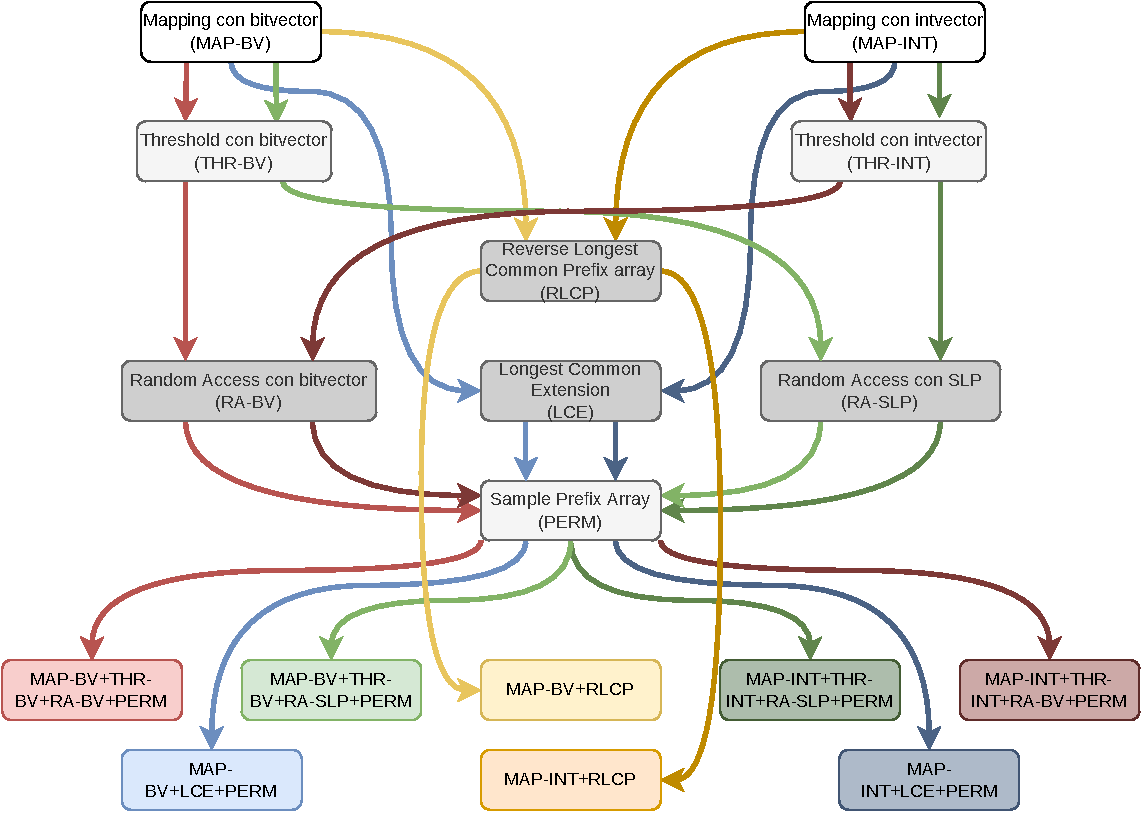
\includegraphics[width=\textwidth]{img/ds.pdf}
  \caption{Schema grafico dell'ottenimento delle otto strutture dati a partire
    dalle varie componenti.}
  \label{fig:compon}
\end{figure}
\subsection{Calcolo degli SMEM con RLCP}
Questa prima soluzione per il calcolo degli $\SMEM$ con un aplotipo esterno è
quella che può essere effettuata tramite le strutture dati composte:
\begin{itemize}
  \item \texttt{MAP-INT + RLCP}
  \item \texttt{MAP-BV + RLCP}
\end{itemize}
I due algoritmi riprendono  quanto discusso per l'algoritmo 5
di Durbin. Tali algoritmi non sfruttano l'uso delle matching statistics e sono
limitati dal non 
poter calcolare quali righe presentano un solo $\SMEM$, calcolando solo quante
siano. Il secondo limite è dato dal fatto che necessitano di avere interamente
in memoria l'$\,\RLCP$ array, una
struttura non run-length encoded.\\
Il metodo procede, quindi, con l'aggiornamento dei tre indici $e_k$, $f_k$ e
$g_k$, avendo che gli ultimi due possono assumere qualsiasi valore in
$\{0,\ldots, M\}$,
come con la $\PBWT$. Avendo memorizzato solo informazioni
relative alle run bisogna, ogni volta, ricondurre gli indici di riga alla
run a cui appartengono.
% Si ricordano quindi i tempi di tale operazione, avendo $r$ numero
% di run per la colonna $k$:
% \begin{itemize}
%   \item con la \texttt{MAP-INT + LCP} si ha tempo proporzionale a:
%   \begin{equation}
%     \label{eq:itrcomp}
%     \mathcal{O}(\log (r))
%   \end{equation}
%   \item con la \texttt{MAP-BV + LCP} si ha tempo proporzionale a:
%   \begin{equation}
%     \label{eq:itrbvcomp}
%     \mathcal{O}\left(\log\frac{M}{r}\right)
%   \end{equation}
% \end{itemize}
Inoltre Durbin sfruttava il random access al pannello in input, avendolo in
memoria insieme al prefix array e al divergence array, al fine di aggiornare il
valore di $e_k$. In entrambe le struttura dati run-length encoded, però,
non si ha in memoria né il prefix array né il pannello ma solo solo la
rappresentazione compatta della matrice $\PBWT$. Quindi, si è dovuto
pensare ad un metodo che ricomponga una data riga $x_j$ del pannello $X$ a
partire da un elemento, indicizzato con $a_{k+1}[i]=j$, con $0\leq i<M$, alla
colonna $k+1$, della 
matrice $\PBWT$. Questo risultato si può ottenere muovendosi da destra a
sinistra, seguendo in modo 
inverso la permutazione che produce il prefix array. In altri termini,
tale metodo permette un mapping inverso, che segue una riga del
pannello originale nella matrice $\PBWT$, a ritroso.\\ 
Per ottenere l'indice alla colonna $k$-esima della matrice $\PBWT$, da cui
proviene la riga $j$, indicizzata all'indice $i$ in
colonna $k+1$ della matrice $\PBWT$, si inizia analizzando il valore
$c[k]$. Infatti, se $i<c[k]$, 
allora sicuramente, in colonna $k$, $i$ è un indice di riga corrispondente a
$\sigma=0$, ricordando come la costruzione della colonna $k+1$
nella matrice $\PBWT$ si abbia grazie ad ordinamento stabile. In caso contrario,
$i$ corrisponde ad un elemento $\sigma=1$ in colonna $k$ della matrice $\PBWT$.
Si sfruttano 
così o l'array $p_k$ o le funzioni 
$\rank_{h_k}$ e $\select_{h_k}$ per risalire all'indice in colonna $k$,
calcolando 
prima l'indice di run e l'eventuale offset, per il quale il mapping porta
all'indice $i'$ in colonna $k+1$, e seguire, virtualmente, la riga $x_j$ del
pannello originale. 
Per quanto riguarda la struttura composta \texttt{MAP-INT + RLCP}, si ha lo
pseudocodice per il 
mapping inverso consultabile all'algoritmo \ref{algo:lfrev} mentre, per quanto
riguarda la struttura composta \texttt{MAP-BV + RLCP}, si ha l'algoritmo
\ref{algo:lfrevbv}. Parlando in termini di complessità in tempo si ha che,
usando la componente \texttt{MAP-INT}, si ha, con $r$ numero di run alla
colonna $k$, un caso peggiore proporzionale a:
\begin{equation}
  \label{eq:revint}
  \mathcal{O}(r)
\end{equation}
Nel caso, invece, in cui si usa la componente \texttt{MAP-BV}, si ha:
\begin{equation}
  \label{eq:revbv}
  \mathcal{O}\left(\log\frac{M}{r}\right)
\end{equation}
\dc{Approfondire?}
\begin{algorithm}
  \begin{algorithmic}[1]
    \Function{reverse\_map}{$k, \,\,i$}
    \Comment $k$ indice di colonna, $i$ indice di riga
    \State \textbf{if} $k=0$ \textbf{then} \textbf{return} $0$
    %\If{$k=0$}
    \Comment by design
    %\State \textbf{return} $0$
    %\EndIf
    \State $k\gets k-1$
    \State $c\gets rlpbwt[k].c$
    \State $u\gets 0$, $v\gets 0$, $offset\gets 0$, $run \gets 0$,
    $found\gets \bot$
    \If {i < c}
    \State $u\gets i$
    \State $prev_0\gets 0$, $next_0\gets 0$
    \For {\textit{every} $j\in [0,|p_k|)$}
    \State $(prev_0,\_) \gets \uvtrick(k,j)$
    \State $(next_0,\_) \gets \uvtrick(k,j+1)$
    \If{$prev_0\leq u<next_0$}
    \State $run\gets j$, $found\gets \top$
    \State \textbf{break}
    \EndIf
    \EndFor
    \State \textbf{if} $\neg found$ \textbf{then} $run \gets |p_k|-1$
    % \If{$\neg found$}
    % \State $run \gets |p_k|-1$
    % \EndIf
    \State $(curr_u,\_)\gets \uvtrick(k, run)$, $offset\gets u-curr_u$
    \State \textbf{return} $p_k[run]+offset$
    \Else

    \State $v\gets i-c$
    \State $prev_1\gets 0$, $next_1\gets 0$
    \For {\textit{every} $j\in [0,|p_k|)$}
    \State $(\_,prev_1) \gets \uvtrick(k,j)$
    \State $(\_,next_1) \gets \uvtrick(k,j+1)$
    \If{$prev_1\leq v<next_1$}
    \State $run\gets j$, $found\gets \top$
    \State \textbf{break}
    \EndIf
    \EndFor
    \State \textbf{if} $\neg found$ \textbf{then} $run \gets |p_k|-1$
    % \If{$\neg found$}
    % \State $run \gets |p_k|-1$
    % \EndIf
    \State $(curr_v,curr_u)\gets \uvtrick(k, run)$, $offset\gets v-curr_v$
    \State \textbf{return} $p_k[run]+offset$
    \EndIf
    \EndFunction
  \end{algorithmic}
  \caption{Algoritmo per il mapping inverso con la \texttt{MAP-INT + RLCP}.}
  \label{algo:lfrev}
\end{algorithm}

\begin{algorithm}
  \begin{algorithmic}[1]
    \Function{reverse\_map}{$k, \,\,i$}
    \Comment $k$ indice di colonna, $i$ indice di riga
    \State \textbf{if} $k=0$ \textbf{then} \textbf{return} $0$
    %\If{$k=0$}
    \Comment by design
    %\State \textbf{return} $0$
    %\EndIf
    \State $k\gets k-1$
    \State $c\gets c[k]$
    \If{$i<c$}
    \If{$start_k$}
    \State $run\gets \rank_u^{k}(i)\cdot 2$
    \Else
    \State $run\gets \rank_u^{k}(i)\cdot 2+1$
    \EndIf
    \State $i_{run}\gets 0$
    \State \textbf{if} $run\neq 0$ \textbf{then} $i_{run}\gets
    \select_h^{k}(run)+1$ 
    % \If{$run\neq 0$}
    % \State $i_{run}\gets select_h^{k}(run)+1$
    % \EndIf
    \State $(prev_0,\,\,\_)\gets \uvtrick(k,\,\,i_{run})$
    \State \textbf{return} $i_{run}+(i-prev_0)$
    \Else
    \If{$start_k$}
    \State $run\gets \rank_v^{k}(i)\cdot 2+1$
    \Else
    \State $run\gets \rank_v^{k}(i)\cdot 2$
    \EndIf
    \State $i_{run}\gets 0$
    \State \textbf{if} $run\neq 0$ \textbf{then} $i_{run}\gets
    \select_h^{k}(run)+1$ 
    % \If{$run\neq 0$}
    % \State $i_{run}\gets select_h^{k}(run)+1$
    % \EndIf
    \State $(\_,\,\,prev_1)\gets \uvtrick(k,\,\,i_{run})$
    \State \textbf{return} $i_{run}+(i-(c+prev_1))$
    \EndIf
    \EndFunction
  \end{algorithmic}
  \caption{Algoritmo per il mapping inverso con la \texttt{MAP-BV + RLCP}.}
  \label{algo:lfrevbv}
\end{algorithm}
Si ha, di conseguenza, un riadattamento dell'algoritmo di Durbin all'uso delle
run, 
ottenendo, ad ogni step, i medesimi valori per $e_k$, $f_k$ e $g_k$. Le uniche
differenze sono:
\begin{itemize}
  \item il calcolo del mapping necessità dell'estrazione dei valori $u$ e $v$,
  tenendo conto esplicito degli offset nel caso della \texttt{MAP-INT + RLCP}
  \item non si ha random access al pannello quindi bisogna procedere,
  ogni volta, con il'inverso del mapping e il calcolo del simbolo a partire
  dall'indice della run
  \item non si ha il prefix array in memoria, quindi non è possibile
  sapere quali siano le righe per le quali si ha uno $\SMEM$ fino alla colonna
  $k$ ma è possibile conoscere solo quante siano, ovvero $g_k-f_k$
\end{itemize}
Anche in questo caso, lo pseudocodice è consultabile all'algoritmo
\ref{algo:matchlcp}. Calcolare la complessità di tale algoritmo non è semplice,
come già visto nel caso dell'algoritmo 5 di Durbin. In modo analogo a quanto
visto per quest'ultimo, si può,
comunque, intuire come i vari cicli interni siano limitati superiormente dalla
larghezza del pannello e dai tempi di mapping. Questo si può stimare in quanto
le occorrenze dei cicli interni sono proporzionali al numero di $\SMEM$ e al
numero 
di step all'indietro necessari a computare il nuovo intervallo. Tale numero di
step scala sul numero di caratteri in overlap tra due $\SMEM$
consecutivi. Fatta questa premessa, si può stimare che il calcolo degli $\SMEM$
con
la struttura \texttt{MAP-INT + RLCP} è proporzionale, con $\rho$ numero medio di
run per una colonna, a:
\begin{equation}
  \label{eq:lcpmatchint}
  \mathcal{O}(N\log \rho)
\end{equation}
Nel caso, invece, della struttura \texttt{MAP-BV + RLCP} si ha:
\begin{equation}
  \label{eq:lcpmatchbv}
  \mathcal{O}\left(N\log\frac{M}{\rho}\right)
\end{equation}
\dc{APPROFONDIRE SPIEGAZIONE ALGORITMI}

\begin{algorithm}
  \footnotesize
  \begin{algorithmic}[1]
    \Function{external\_matches}{$z$}
    \Comment si assume $|z|=N$
    \State $f\gets 0,\,\,f_{run}\gets 0,\,\,f'\gets 0$
    \State $g\gets 0,\,\,g_{run}\gets 0,\,\,g'\gets 0$
    \State $e\gets 0,\,\,nh\gets 0$
    \For {\textit{every} $k\in\left[0,\,\, |z|\right)$}
    \State $f_{run}\gets \ITR(f,k)$ \textbf{oppure} $f_{run}\gets
    \rank_h^k(f)$ 
    \State $g_{run}\gets \ITR(g,k)$ \textbf{oppure} $f_{run}\gets
    \rank_h^k(g)$ 
    \State $f'\gets \W(k,\,\, f,\,\, z[k]),\,\,g'\gets \W(k,\,\,
    g,\,\, z[k]),\,\,nh\gets g-f$
    \If{$f'<g'$}
    \State $f\gets f',\,\,g\gets g'$
    \Else
    \If{$k\neq 0$}
    %\State \textbf{report} \textit{matches in} $[e,\,\, k-1]$ \textit{with} $l$
    \State \textit{memorizzazione degli SMEM tra le colonne} $[e,\,\, k-1]$
    \textit{con} $nh$ aplotipi
    \EndIf
    \State \textbf{if} $f'=|l_{k+1}|$ \textbf{then} $e\gets k+1$ \textbf{else}
    $e\gets k-l_{k+1}[f']$ 
    % \If {$f'=|l_{k+1}|$}
    % \State $e\gets k+1$
    % \Else
    % \State  $e\gets k-l_{k+1}[f']$
    % \EndIf
    \If{$(z[e]=0\land f'>0)\lor f'=M$}
    \State $f'\gets g'-1$
    \If{$e\geq 1$}
    \State $f_{rev}\gets f',\,\,k'\gets k+1$
    \While { $k'\neq e-1$}
    \State  $f_{rev}\gets \RM(k',\,\,f_{rev}),\,\,k'\gets k'-1$
    \EndWhile
    \State $run\gets \ITR(f_{rev},k')$ \textbf{oppure} $run\gets
    \rank_h^{k'}(f_{rev})$
    \State $symb\gets \GS(start_{k'}, run)$ 
    \While {$e>0\land z[e-1]=symb$}
    \State $e\gets e-1,\,\,f_{rev}\gets \RM(e, \,\,f_{rev})$
    \State $run\gets \ITR(f_{rev}, e-1)$ \textbf{oppure} $run\gets
    \rank_h^{e-1}(f_{rev})$
    \State $symb\gets \GS(start_{e-1}, run)$ 
    \EndWhile
    \EndIf
    \State \textbf{while} $f'>0\land (k+1)-l_{k+1}[f]\leq e$ \textbf{do}
    $f'\gets f'-1$ 
    \State $f\gets f',\,\,g\gets g'$
    \Else
    \State $g'\gets f'-1$
    \If{$e\geq 1$}
    \State $f_{rev}\gets f',\,\,k'\gets k+1$
    \While {$k'\neq e-1$}
    \State  $f_{rev}\gets \RM(k',\,\,f_{rev}),\,\,k'\gets k'-1$
    \EndWhile
    \State $run\gets \ITR(f_{rev},k')$ \textbf{oppure} $run\gets
    \rank_h^{k'}(f_{rev})$
    \State $symb\gets \GS(start_{k'}, 
    run)$ 
    \While {$e>0\land z[e-1]=symb$}
    \State $e\gets e-1,\,\,f_{rev}\gets \RM(e, \,\,f_{rev})$
    \State $run\gets \ITR(f_{rev},e-1)$ \textbf{oppure} $run\gets
    \rank_h^{e-1}(f_{rev})$
    \State $symb\gets \GS(start_{e-1}, run)$ 
    \EndWhile
    \EndIf
    \State \textbf{while} $e<M\land (k+1)-l_{k+1}[g']\leq e$ \textbf{do}
    $g'\gets g'+1$  
    \State $f\gets f',\,\,g\gets g'$
    \EndIf
    \EndIf
    \EndFor
    \If{$f<g$}
    \State $nh\gets g-f$
    \State \textit{memorizzazione degli SMEM tra le colonne} $[e,\,\, |z|-1]$
    \textit{con} $nh$ aplotipi
    \EndIf
    \EndFunction
  \end{algorithmic}
  \caption{\footnotesize{Calcolo degli SMEM con aplotipo esterno per
  \texttt{MAP-INT/BV + RLCP}, con eventuali usi diversificati per
  \texttt{MAP-INT} e \texttt{MAP-BV} segnalati con ``oppure''.}} 
  \label{algo:matchlcp}
\end{algorithm}


% \begin{algorithm}
%   \footnotesize
%   \begin{algorithmic}[1]
%     \Function{external\_matches}{$z$}
%     \Comment $|z|=N$
%     \State $f\gets 0,\,\,f_{run}\gets 0,\,\,f'\gets 0$
%     \State $g\gets 0,\,\,g_{run}\gets 0,\,\,g'\gets 0$
%     \State $e\gets 0,\,\,nh\gets 0$
%     \For {\textit{every} $k\in\left[0,\,\, |z|\right)$}
%     \State $f_{run}\gets rank_h^k(f),\,\,g_{run}\gets rank_h^k(g)$
%     \State $f'\gets w(k,\,\, f,\,\, z[k]),\,\,g'\gets w(k,\,\, g,\,\, z[k])$
%     \State $nh\gets g-f$
%     \If{$f'<g'$}
%     \State $f\gets f',\,\,g\gets g'$
%     \Else
%     \If{$k\neq 0$}
%     \State \textit{memorizzazione degli SMEM tra le colonne} $[e,\,\, k-1]$
%     \textit{con} $nh$ aplotipi
%     \EndIf
%     \If{$f'=|l_{k+1}|$}
%     \State $e\gets k+1$
%     \Else
%     \State $e\gets k-l_{k+1}[f']$
%     \EndIf
    
%     \If{$(z[e]=0\land f'>0)\lor f'=M$}
%     \State $f'\gets g'-1$
%     \If{$e\geq 1$}
%     \State $f_{rev}\gets f',\,\,k'\gets k+1$
%     \While {$k'\neq e-1$}
%     \State $f_{rev}\gets reverse\_map(k', \,\,f_{rev}),\,\,k'\gets k'-1$
%     \EndWhile
%     \State $run\gets rank_h^{k'}(f_{rev}),\,\,symb\gets get\_symbol(start_{k'},
%     run)$ 
%     \While {$e>0\land z[e-1]=symb$}
%     \State $f_{rev}\gets reverse\_map(e, \,\,f_{rev})$
%     \State $run\gets rank_h^{e-1}(f_{rev})$
%     \State $symb\gets get\_symbol(start_{e-1}, run)$
%     \EndWhile
%     \EndIf
%     \State \textbf{while} $f'>0\land (k+1)-l_{k+1}[f]\leq e$ \textbf{do}
%     $e\gets e-1$ 
%     \State $f\gets f',\,\,g\gets g'$
%     \Else
%     \State $g'\gets f'-1$
%     \If{$e\geq 1$}
%     \State $f_{rev}\gets f',\,\,k'\gets k+1$
%     \While {$k'\neq e-1$}
%     \State $f_{rev}\gets reverse\_map(k', \,\,f_{rev}),\,\,k'\gets k'-1$
%     \EndWhile
%     \State $run\gets rank_h^{k'}(f_{rev}),\,\,symb\gets get\_symbol(start_{k'},
%     run)$ 
%     \While {$e>0\land z[e-1]=symb$}
%     \State $f_{rev}\gets reverse\_map(e, \,\,f_{rev})$
%     \State $run\gets rank_h^{e-1}(f_{rev})$
%     \State $symb\gets get\_symbol(start_{e-1}, run)$
%     \EndWhile
%     \EndIf
%     \State \textbf{while} $e<M\land (k+1)-l_{k+1}[e]\leq e$ \textbf{do}
%     $e\gets e+1$  
%     \State $f\gets f',\,\,g\gets g'$
%     \EndIf
%     \EndIf
%     \EndFor
%     \If{$f<g$}
%     \State $nh\gets g-f$
%     \State \textit{memorizzazione degli SMEM tra le colonne} $[e,\,\, |z|-1]$
%     \textit{con} $nh$ aplotipi  
%     \EndIf
%     \EndFunction
%   \end{algorithmic}
%   \caption{\footnotesize{Calcolo degli SMEM con aplotipo esterno per
%   \texttt{MAP-BV + LCP}.}} 
%   \label{algo:matchpanelbv}
% \end{algorithm}